\documentclass[aspectratio=169,10pt]{beamer}
\usepackage[utf8]{inputenc}
\usepackage[T1]{fontenc}
\usepackage{amsmath,amssymb}
\usepackage{booktabs}
\usepackage{colortbl}
\usepackage{xcolor}
\usepackage{tikz}
\usepackage{listings}
\usepackage{microtype}
\usepackage{array}
\usepackage{tcolorbox}
\tcbuselibrary{skins,breakable}

% ── Red/DarkRed Theme (Original) ─────────────────────────────────
\definecolor{darkred}{RGB}{180,30,30}
\definecolor{hlblue}{RGB}{220,235,255}
\definecolor{hlgreen}{RGB}{220,245,220}
\definecolor{codebg}{RGB}{245,245,250}
\definecolor{steelblue}{RGB}{70,130,180}
\definecolor{Navy}{RGB}{18,32,68}
\definecolor{Coral}{RGB}{214,80,60}
\definecolor{Slate}{RGB}{90,100,120}
\definecolor{Rule}{RGB}{210,213,220}
\definecolor{CodeBg}{RGB}{248,249,251}
\definecolor{TblHead}{RGB}{180,30,30}
\definecolor{TblAlt}{RGB}{252,240,240}
\definecolor{GreenOk}{RGB}{34,120,60}
\definecolor{Amber}{RGB}{180,110,0}

% ── Beamer setup with red theme ─────────────────────────────────
\usetheme{CambridgeUS}
\usecolortheme{beaver}
\setbeamertemplate{navigation symbols}{}

% Red block styling
\setbeamertemplate{blocks}[rounded][shadow=true]
\setbeamercolor{block title}{bg=darkred!85,fg=white}
\setbeamercolor{block body}{bg=darkred!5,fg=black}

% Red item bullets
\setbeamertemplate{itemize item}{\textcolor{darkred}{\textbullet}}
\setbeamertemplate{itemize subitem}{\textcolor{darkred}{--}}
\setlength{\leftmargini}{1.2em}

% ── Frame title with red bar ────────────────────────────────────
\setbeamertemplate{frametitle}{%
  \vspace{0.5em}%
  \begin{tikzpicture}[overlay,remember picture]
    \fill[darkred]
      ([xshift=0.52cm,yshift=-0.06cm]current page.north west)
      rectangle
      ([xshift=0.80cm,yshift=-0.96cm]current page.north west);
  \end{tikzpicture}%
  \hspace{0.62cm}%
  {\usebeamerfont{frametitle}\usebeamercolor[fg]{frametitle}%
   \insertframetitle}%
  \ifx\insertframesubtitle\empty\else\\[0.08em]%
    \hspace{0.62cm}{\small\textcolor{Slate}{\textit{\insertframesubtitle}}}%
  \fi%
}

% ── Footline with red theme ─────────────────────────────────────
\setbeamertemplate{footline}{%
  \leavevmode%
  \hbox{%
    \begin{beamercolorbox}[wd=.40\paperwidth,ht=2.25ex,dp=1ex,center]{author in head/foot}%
      \usebeamerfont{author in head/foot}\insertshortauthor
    \end{beamercolorbox}%
    \begin{beamercolorbox}[wd=.40\paperwidth,ht=2.25ex,dp=1ex,center]{title in head/foot}%
      \usebeamerfont{title in head/foot}\insertshorttitle
    \end{beamercolorbox}%
    \begin{beamercolorbox}[wd=.20\paperwidth,ht=2.25ex,dp=1ex,right]{date in head/foot}%
      \insertframenumber{} / \inserttotalframenumber\hspace*{2ex}
    \end{beamercolorbox}%
  }%
  \vskip0pt%
}

% ── Code style ──────────────────────────────────────────────────
\lstdefinestyle{paper}{
  language=Python,
  backgroundcolor=\color{CodeBg},
  basicstyle=\ttfamily\fontsize{7}{9}\selectfont,
  keywordstyle=\color{steelblue}\bfseries,
  commentstyle=\color{Slate}\itshape,
  stringstyle=\color{Coral},
  numbers=left, numberstyle=\tiny\color{Rule}, numbersep=5pt,
  frame=none, breaklines=true, showstringspaces=false,
  xleftmargin=8pt, xrightmargin=4pt,
  aboveskip=0pt, belowskip=0pt,
}
\lstset{style=paper}

% ── Helpers ─────────────────────────────────────────────────────
\newcommand{\hruleslide}{%
  \vspace{0.15em}{\color{Rule}\hrule height 0.4pt}\vspace{0.3em}}

\newcommand{\thead}[1]{%
  \cellcolor{TblHead}\textcolor{white}{\textbf{\footnotesize #1}}}
\newcommand{\talt}{\rowcolor{TblAlt}}

\newcommand{\ptag}[2]{%
  \tikz[baseline=(t.base)]\node[fill=#1,rounded corners=2pt,
  inner xsep=4pt, inner ysep=1.5pt,text=white,
  font=\bfseries\fontsize{6}{7}\selectfont](t){#2};}

\newcommand{\notebox}[2]{%
  \begin{tcolorbox}[colback=#1!5,colframe=#1!80,boxrule=0.5pt,arc=2pt,left=2pt,right=2pt,top=2pt,bottom=2pt]
    \footnotesize\textcolor{#1!80!black}{\bfseries Note}\enspace #2
  \end{tcolorbox}}

% ── Metadata ────────────────────────────────────────────────────
\title[LLM Uncertainty Bench]{Benchmarking LLMs via Uncertainty Quantification}
\author[Ye et al., NeurIPS 2024]{%
  Fanghua Ye \and Mingming Yang \and Jianhui Pang \and Longyue Wang \\[2pt]
  Derek F.\ Wong \and Emine Yilmaz \and Shuming Shi \and Zhaopeng Tu}
\institute{Tencent AI Lab \quad $\cdot$ \quad UCL \quad $\cdot$ \quad University of Macau}
\date{NeurIPS 2024 \,--\, Datasets and Benchmarks Track}

% ============================================================
\begin{document}
% ============================================================

% ── footline ────────────────────────────────────────────────────
\setbeamertemplate{footline}{%
  \leavevmode%
  \hbox{%
    \begin{beamercolorbox}[wd=.40\paperwidth,ht=2.25ex,dp=1ex,center]{author in head/foot}%
      \usebeamerfont{author in head/foot}\insertshortauthor
    \end{beamercolorbox}%
    \begin{beamercolorbox}[wd=.40\paperwidth,ht=2.25ex,dp=1ex,center]{title in head/foot}%
      \usebeamerfont{title in head/foot}\insertshorttitle
    \end{beamercolorbox}%
    \begin{beamercolorbox}[wd=.20\paperwidth,ht=2.25ex,dp=1ex,right]{date in head/foot}%
      \insertframenumber{} / \inserttotalframenumber\hspace*{2ex}
    \end{beamercolorbox}%
  }%
  \vskip0pt%
}

% ── metadata ────────────────────────────────────────────────────
\title[LLM Uncertainty Bench]{Benchmarking LLMs via Uncertainty Quantification}
\author[Ye et al., NeurIPS 2024]{%
  Fanghua Ye \and Mingming Yang \and Jianhui Pang \and Longyue Wang \\[2pt]
  Derek F.\ Wong \and Emine Yilmaz \and Shuming Shi \and Zhaopeng Tu}
\institute{Tencent AI Lab \quad $\cdot$ \quad UCL \quad $\cdot$ \quad University of Macau}
\date{NeurIPS 2024 \,--\, Datasets and Benchmarks Track}

% ── helpers ─────────────────────────────────────────────────────
\newcommand{\hrow}{\rowcolor{hlblue}}
\newcommand{\grow}{\rowcolor{hlgreen}}

% \begin{document}

\maketitle
% ================================================================
% Q1 — PROMPTING STRATEGIES 
% ================================================================
\begin{frame}{Q1\enspace What is a Prompting Strategy?}



\vspace{0.5em}
\begin{columns}[T]
  \begin{column}{0.31\textwidth}
    {\small\bfseries\color{darkred}\ptag{darkred}{01}\enspace Base Prompt}
    \vspace{0.4em}

    {\footnotesize Minimal format, just question + choices + ``Answer:''}
    \vspace{0.5em}

    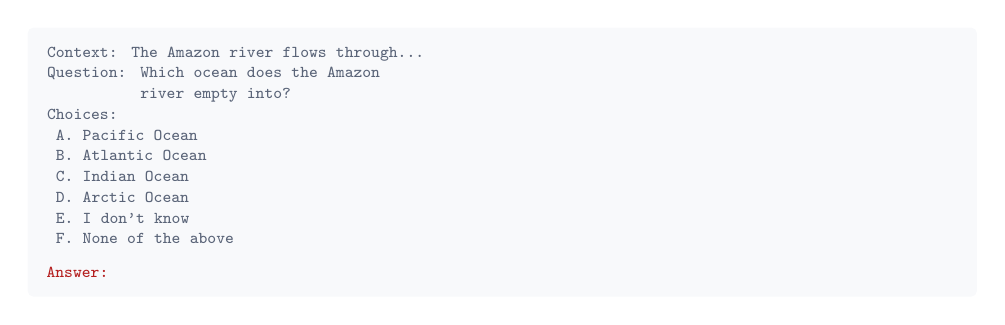
\begin{tikzpicture}
      \node[fill=CodeBg,inner sep=7pt,rounded corners=2pt,
            text width=\linewidth-16pt,align=left]{%
        \ttfamily\fontsize{6}{7.5}\selectfont\color{Slate}
        Context: The Amazon river flows through...\\
        Question: Which ocean does the Amazon\\
        \phantom{Question: }river empty into?\\
        Choices:\\
        \phantom{C}A. Pacific Ocean\\
        \phantom{C}B. Atlantic Ocean\\
        \phantom{C}C. Indian Ocean\\
        \phantom{C}D. Arctic Ocean\\
        \phantom{C}E. I don't know\\
        \phantom{C}F. None of the above\\
        \textbf{\textcolor{darkred}{Answer:}}
      };
    \end{tikzpicture}
  \end{column}

  \begin{column}{0.01\textwidth}\color{Rule}\vrule\end{column}

  \begin{column}{0.31\textwidth}
    {\small\bfseries\color{darkred}\ptag{darkred}{02}\enspace Shared Instruction}
    \vspace{0.4em}

    {\footnotesize Adds a generic task description at the top}
    \vspace{0.5em}

    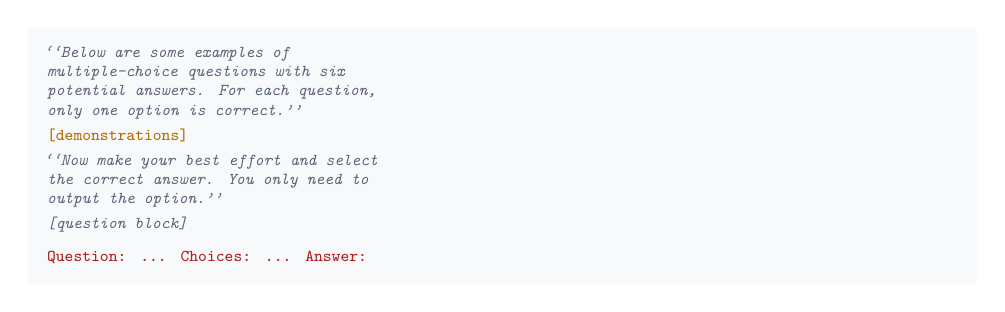
\begin{tikzpicture}
      \node[fill=CodeBg,inner sep=7pt,rounded corners=2pt,
            text width=\linewidth-16pt,align=left]{%
        \ttfamily\fontsize{5.8}{7}\selectfont\color{Slate}
        \textit{``Below are some examples of}\\
        \textit{multiple-choice questions with six}\\
        \textit{potential answers. For each question,}\\
        \textit{only one option is correct.''}\\[2pt]
        \textcolor{Amber}{[demonstrations]}\\[2pt]
        \textit{``Now make your best effort and select}\\
        \textit{the correct answer. You only need to}\\
        \textit{output the option.''}\\[2pt]
        \textit{[question block]}\\
        \textbf{\textcolor{darkred}{Question: ... Choices: ... Answer:}}
      };
    \end{tikzpicture}
  \end{column}

  \begin{column}{0.01\textwidth}\color{Rule}\vrule\end{column}

  \begin{column}{0.31\textwidth}
    {\small\bfseries\color{darkred}\ptag{darkred}{03}\enspace Task-Specific}
    \vspace{0.4em}

    {\footnotesize Adds a task-tailored description. For DS: ``the answer is the option that accurately summarizes the document without hallucination.''}
    \vspace{0.5em}

    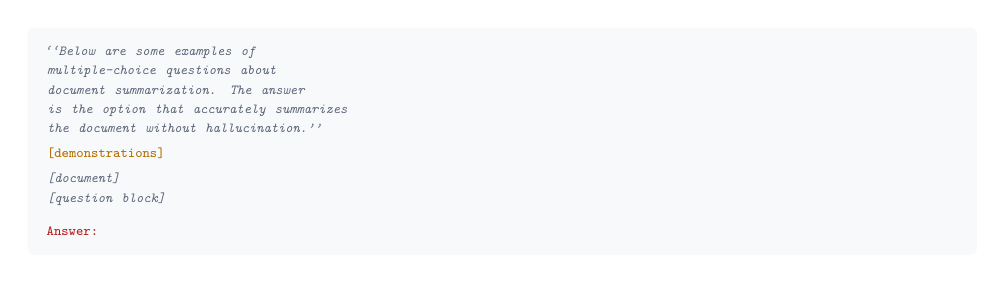
\begin{tikzpicture}
      \node[fill=CodeBg,inner sep=7pt,rounded corners=2pt,
            text width=\linewidth-16pt,align=left]{%
        \ttfamily\fontsize{5.5}{7}\selectfont\color{Slate}
        \textit{``Below are some examples of}\\
        \textit{multiple-choice questions about}\\
        \textit{document summarization. The answer}\\
        \textit{is the option that accurately summarizes}\\
        \textit{the document without hallucination.''}\\[2pt]
        \textcolor{Amber}{[demonstrations]}\\[2pt]
        \textit{[document]}\\
        \textit{[question block]}\\
        \textbf{\textcolor{darkred}{Answer:}}
      };
    \end{tikzpicture}
  \end{column}
\end{columns}

\vspace{0.45em}\hruleslide
{\footnotesize\color{Slate}
  \textbf{Key insight:} LLMs are sensitive to prompt phrasing — the same model can give different probability distributions depending on how the question is formatted. Averaging results across all three strategies makes the benchmark fairer.}
\end{frame}

% ================================================================
% Q2 — FIVE TASKS (UPDATED WITH EXAMPLES)
% ================================================================
\begin{frame}{Q2\enspace The Five Tasks with Concrete Examples}


\vspace{0.2em}
\begin{columns}[T]
  \begin{column}{0.48\textwidth}
    {\small\bfseries\color{darkred}Question Answering (QA)} — MMLU
    \vspace{0.2em}
    \begin{tcolorbox}[colback=CodeBg,colframe=Rule,boxrule=0.4pt,arc=2pt,left=2pt,right=2pt,top=2pt,bottom=2pt,fontupper=\tiny]
      \textit{What is the powerhouse of the cell?}\\
      A. Nucleus \qquad B. Mitochondria\\
      C. Ribosome \qquad D. Golgi apparatus\\
      E. I don't know \quad F. None of the above\\
      {\color{GreenOk}\bfseries Answer: B}
    \end{tcolorbox}
    
    {\small\bfseries\color{darkred}Reading Comprehension (RC)} — CosmosQA
    \vspace{0.2em}
    \begin{tcolorbox}[colback=CodeBg,colframe=Rule,boxrule=0.4pt,arc=2pt,left=2pt,right=2pt,top=2pt,bottom=2pt,fontupper=\tiny]
      \textit{Context: ``I burnt my hand while cooking dinner. I had to go to the ER. The doctor said it was a second-degree burn.''}\\
      \textit{What is likely true about this person?}\\
      A. They enjoy extreme sports \quad B. Will need follow-up care\\
      C. Professional chef \qquad \;\; D. Trying to hurt themselves\\
      E. I don't know \quad F. None of the above\\
      {\color{GreenOk}\bfseries Answer: B}
    \end{tcolorbox}
    
    {\small\bfseries\color{darkred}Commonsense Inference (CI)} — HellaSwag
    \vspace{0.2em}
    \begin{tcolorbox}[colback=CodeBg,colframe=Rule,boxrule=0.4pt,arc=2pt,left=2pt,right=2pt,top=2pt,bottom=2pt,fontupper=\tiny]
      \textit{Context: ``A man is pouring cement into a mold.''}\\
      \textit{Which ending is most likely?}\\
      A. Waters the plants \quad B. Waits for it to dry\\
      C. Paints the walls \quad D. Throws mold into river\\
      E. I don't know \quad F. None of the above\\
      {\color{GreenOk}\bfseries Answer: B}
    \end{tcolorbox}
  \end{column}

  \begin{column}{0.02\textwidth}\color{Rule}\vrule\end{column}

  \begin{column}{0.48\textwidth}
    {\small\bfseries\color{darkred}Dialogue Response Selection (DRS)} — HaluDial
    \vspace{0.2em}
    \begin{tcolorbox}[colback=CodeBg,colframe=Rule,boxrule=0.4pt,arc=2pt,left=2pt,right=2pt,top=2pt,bottom=2pt,fontupper=\tiny]
      \textit{User: ``Who directed Inception?''}\\
      \textit{Bot: ``Christopher Nolan directed Inception.''}\\
      \textit{User: ``What other movies has he made?''}\\
      \textit{Which response is most appropriate?}\\
      A. Titanic and Avatar \quad B. Dark Knight, Interstellar\\
      C. He is a novelist \quad D. Only one film\\
      E. I don't know \quad F. None of the above\\
      {\color{GreenOk}\bfseries Answer: B}
    \end{tcolorbox}
    
    {\small\bfseries\color{darkred}Document Summarization (DS)} — HaluSum
    \vspace{0.2em}
    \begin{tcolorbox}[colback=CodeBg,colframe=Rule,boxrule=0.4pt,arc=2pt,left=2pt,right=2pt,top=2pt,bottom=2pt,fontupper=\tiny]
      \textit{[CNN article about European flooding]}\\
      \textit{Which best summarizes the document?}\\
      A. Drought hit Spain \quad B. Severe floods hit Europe\\
      C. Leaders met on climate \quad D. Hurricane struck Portugal\\
      E. I don't know \quad F. None of the above\\
      {\color{GreenOk}\bfseries Answer: B}
    \end{tcolorbox}
    
    \vspace{0.3em}
    {\footnotesize\color{Slate}
      \textbf{Note:} HaluDial and HaluSum originally had only 2 options. The authors added 2 random distractors from other instances + options E and F to reach 6 options total, standardizing difficulty across all tasks.}
  \end{column}
\end{columns}
\end{frame}

% ================================================================
% Q3 — SOFTMAX / LOGIT EXTRACTION
% ================================================================
\begin{frame}[fragile]{Q3\enspace Softmax Probability Extraction}

\begin{columns}[T]
  \begin{column}{0.40\textwidth}
    \vspace{0.2em}
    {\small\bfseries\color{darkred}Steps }
    \hruleslide
    \begin{enumerate}\setlength\itemsep{5pt}\footnotesize
      \item Feed the full formatted prompt (ending with \texttt{Answer:}) to the LLM
      \item The LLM's \textbf{language modelling head} produces logits over the full vocabulary at the \emph{last} token position
      \item Extract only the logits corresponding to the \textbf{six option letters} A, B, C, D, E, F
      \item Apply the \textbf{softmax function} over those 6 logits only $\Rightarrow$ restricted probability vector $\mathbf{p}\in\mathbb{R}^6$, $\sum p_k=1$
    \end{enumerate}

    \vspace{0.7em}
    \notebox{Coral}{Requires direct access to model logits. Not available for closed-source APIs (GPT-4 etc.). The paper approximates via sampling 50 answers and computing option frequencies.}
  \end{column}

  \begin{column}{0.57\textwidth}
    \begin{lstlisting}
# Tokenise and run one forward pass
ids = tokenizer(prompt, return_tensors="pt")
with torch.no_grad():
    out = model(**ids)

# Logits at LAST token position [vocab_size]
last_logits = out.logits[0, -1, :]

# Token IDs for the six option letters
option_ids = [
    tokenizer("A").input_ids[-1],
    tokenizer("B").input_ids[-1],
    tokenizer("C").input_ids[-1],
    tokenizer("D").input_ids[-1],
    tokenizer("E").input_ids[-1],
    tokenizer("F").input_ids[-1],
]

# Restricted softmax over 6 logits only
probs = torch.softmax(
    last_logits[option_ids], dim=0)
# e.g. [0.60, 0.25, 0.08, 0.04, 0.02, 0.01]
#        A      B     C     D     E     F
    \end{lstlisting}
    \vspace{0.2em}
    {\fontsize{7}{9}\selectfont\color{Slate}
      The softmax is computed only over the 6 option-letter tokens, not the full vocabulary.}
  \end{column}
\end{columns}
\end{frame}

% ================================================================
% Q4 — MEAN OF LAC AND APS
% ================================================================
\begin{frame}{Q4\enspace Mean of LAC and APS in the Tables}


\vspace{0.1em}
\begin{columns}[T]
  \begin{column}{0.46\textwidth}
    {\small\bfseries\color{darkred}LAC — Least Ambiguous Classifier \normalfont\small(Sadinle et al., 2019)}
    \hruleslide
    \[s(X,Y)=1-f(X)_Y\]
    {\footnotesize
      Score = 1 minus the softmax probability of the \emph{true label} $Y$ only.\\[4pt]
      Prediction set includes all $Y'$ where $f(X)_{Y'}\!\geq\!1-\hat{q}$.\\[4pt]
      \textcolor{GreenOk}{$\Rightarrow$ Smallest average set size (provably optimal).}\\
      \textcolor{Coral}{$\Rightarrow$ May undercover hard instances.}\\[4pt]
      \textcolor{Slate}{\small``LAC can lead to prediction sets with the smallest average size.}
    }
  \end{column}

  \begin{column}{0.02\textwidth}\color{Rule}\vrule\end{column}

  \begin{column}{0.46\textwidth}
    {\small\bfseries\color{darkred}APS — Adaptive Prediction Sets \normalfont\small(Romano et al., 2020)}
    \hruleslide
    \[s(X,Y)=\!\!\sum_{\substack{Y'\in\mathcal{Y}:\\f(X)_{Y'}\geq f(X)_Y}}\!\!f(X)_{Y'}\]
    {\footnotesize
      Accumulates ranked softmax scores from the top down to the true label.\\[4pt]
      \textcolor{GreenOk}{$\Rightarrow$ Addresses LAC's limitation on hard instances.}\\
      \textcolor{Coral}{$\Rightarrow$ Larger sets on average.}\\[4pt]
      \textcolor{Slate}{\small``APS leverages the softmax scores of all labels, not just the true label.}
    }
  \end{column}
\end{columns}

\vspace{0.55em}\hruleslide

{\footnotesize\bfseries\color{darkred}Why average?}\enspace
{\footnotesize\color{Slate}
  ``APS can lead to a significantly different ranking of LLMs based on uncertainty compared to LAC.
  For example, on the CI task, Qwen-14B secures the lowest uncertainty under LAC but is ranked sixth under APS.
  It is essential to average the two score functions to provide a more accurate quantification of uncertainty.}
\end{frame}

% ================================================================
% Q5 — OVERCOVERAGE
% ================================================================
\begin{frame}{Q5\enspace Overcoverage — Why 92.94\% Instead of 90\%?}

\begin{columns}[T]
  \begin{column}{0.46\textwidth}
    {\small\bfseries\color{darkred}What the paper states}
    \hruleslide
    \begin{itemize}\setlength\itemsep{5pt}\footnotesize
      \item \textbf{Finite-sample correction .}
        The threshold uses the $\frac{\lceil(n+1)(1-\alpha)\rceil}{n}$ quantile, which is always slightly above $1-\alpha$ to ensure the guarantee.
      \item \textbf{Minor fluctuations .}
        ``While the theoretical guarantee is rigorous, there can be minor fluctuations in practice due to finite-sample variability.''
      \item \textbf{LAC vs.\ APS difference.}
        ``APS tends to achieve higher coverage rates than LAC due to its larger prediction sets.'' (Appendix C.1). Their average inflates combined coverage.
    \end{itemize}
  \end{column}

  \begin{column}{0.02\textwidth}\color{Rule}\vrule\end{column}

  \begin{column}{0.46\textwidth}
    {\small\bfseries\color{darkred}How to reduce overcoverage}
    {\footnotesize\color{Slate}\itshape (from conformal prediction literature, not stated in paper)}
    \hruleslide
    \begin{itemize}\setlength\itemsep{5pt}\footnotesize
      \item \textbf{RAPS} (Angelopoulos et al., 2020).
        Adds rank penalty $\lambda\cdot(o(Y)-k_{\text{reg}})^+$ to APS score. Discourages large sets.
      \item \textbf{SAPS.}
        Uses rank-based rather than cumulative probability scores. Reduces sensitivity to miscalibration.
      \item \textbf{Temperature scaling.}
        Recalibrates softmax with scalar $T$ fitted on calibration data $\Rightarrow$ tighter conformal scores.
      \item \textbf{Mondrian CP.}
        Separate thresholds per difficulty stratum to avoid overcovering easy instances.
    \end{itemize}
  \end{column}
\end{columns}

\vspace{0.45em}\hruleslide
{\footnotesize\color{Slate}
  Overcoverage is conservative (safe) but inflates SS, making uncertainty appear higher than it truly is.
  All models achieve average CR $\geq90\%$; the lowest individual CR is 89.56\% (Qwen-7B on DS).}
\end{frame}

% ================================================================
% Q6 — CALIBRATION & SET SIZE
% ================================================================
\begin{frame}{Q6\enspace Calibration of Softmax Probabilities}

\begin{columns}[T]
  \begin{column}{0.42\textwidth}
    {\small\bfseries\color{darkred}ECE Results — InternLM-7B (Table 3)}\\
    {\fontsize{7.5}{9}\selectfont\color{Slate}Expected Calibration Error (\%) — lower is better}
    \vspace{0.35em}

    \renewcommand{\arraystretch}{1.42}
    \begin{tabular}{@{}lrrr@{}}
    \thead{Task} & \thead{CP} & \thead{Entropy} & \thead{$P_{\max}$} \\
    \talt QA  & 15.83 & 15.83 & 15.83 \\
         RC  & \textcolor{GreenOk}{\bfseries 1.33}  & 1.32  & 1.41  \\
    \talt CI  & \textcolor{GreenOk}{\bfseries 3.16}  & 3.45  & 3.75  \\
         DRS & \textcolor{GreenOk}{\bfseries 12.11} & 12.40 & 12.45 \\
    \talt DS  & 9.30  & 9.30  & 9.62  \\
    \midrule
    \textbf{Avg} & \textcolor{GreenOk}{\bfseries 8.35} & 8.46 & 8.61 \\
    \end{tabular}

    \vspace{0.5em}
    {\footnotesize\color{Slate}
      ``Conformal prediction yields the lowest average ECE score, suggesting that it offers more reliable uncertainty quantification.}
  \end{column}

  \begin{column}{0.02\textwidth}\color{Rule}\vrule\end{column}

  \begin{column}{0.50\textwidth}
    {\small\bfseries\color{darkred}Link: calibration $\leftrightarrow$ set size}
    \hruleslide
    \begin{itemize}\setlength\itemsep{5pt}\footnotesize
      \item Raw softmax scores \textbf{usually do not reflect the true class distribution} due to over- or under-confident model predictions. (§3)
      \item CP \textbf{converts any heuristic uncertainty} into a statistically rigorous one via the calibration set — coverage holds regardless of raw calibration quality. (§3)
      \item \textbf{Good calibration} $\Rightarrow$ informative scores $\Rightarrow$ smaller SS.
      \item \textbf{Overconfident} softmax $\Rightarrow$ inflated scores even for wrong answers $\Rightarrow$ LAC threshold rises $\Rightarrow$ larger SS.
      \item \textbf{Underconfident} softmax $\Rightarrow$ diffuse $\mathbf{p}$ $\Rightarrow$ APS cumulative sum reaches $\hat{q}$ quickly $\Rightarrow$ larger SS.
    \end{itemize}

    \vspace{0.4em}
    \notebox{GreenOk}{SS is statistically calibrated by construction (coverage guarantee). Entropy and $P_{\max}$ simply reflect the raw softmax.}
  \end{column}
\end{columns}
\end{frame}

% ================================================================
% Q7 — ENTROPY, PERPLEXITY, SS
% ================================================================
\begin{frame}{Q7\enspace Entropy, Perplexity \& Set Size}

\begin{columns}[T]
  \begin{column}{0.46\textwidth}
    {\small\bfseries\color{darkred}Measures of uncertainty from $\mathbf{p}$}
    \hruleslide

    \textbf{\footnotesize Shannon Entropy}
    \[H(\mathbf{p})=-\sum_k p_k\log_2 p_k\;\in[0,\log_2 K]\]
    {\footnotesize\color{Slate}$H=0$: certain. $H=\log_2 6\approx2.58$\,bits: uniform = maximally uncertain.}

    \vspace{0.5em}
    \textbf{\footnotesize Perplexity (used in paper as baseline, §6.6)}
    \[\mathrm{PPL}=2^H\;\in[1,K]\]
    {\footnotesize\color{Slate}
      ``Perplexity takes values in the range $[1,|\mathcal{Y}|]$, allowing it to be interpreted as prediction set size.'' (§6.6)\\[3pt]
      ``When the predicted probability for each class is $1/|\mathcal{Y}|$, $\mathrm{PPL}=|\mathcal{Y}|$.}

  \end{column}

  \begin{column}{0.02\textwidth}\color{Rule}\vrule\end{column}

  \begin{column}{0.46\textwidth}
    {\small\bfseries\color{darkred}Why CP (SS) dominates PPL}
    \hruleslide

    {\footnotesize\bfseries\color{darkred}From Table 2 — InternLM-7B:}
    \vspace{0.3em}

    \renewcommand{\arraystretch}{1.35}
    {\fontsize{7.5}{9.5}\selectfont
    \begin{tabular}{@{}lrrrr@{}}
    \thead{Task} & \thead{CR\,CP} & \thead{CR\,PPL} & \thead{SS\,CP} & \thead{SS\,PPL} \\
    \talt QA  & \textbf{90.68} & \textcolor{Coral}{83.44} & 3.49 & 2.89 \\
         DRS & \textbf{90.40} & \textcolor{Coral}{86.80} & 3.63 & 3.42 \\
    \talt DS  & \textbf{90.34} & \textcolor{Coral}{87.13} & 4.47 & 4.33 \\
         Avg & \textbf{90.96} & 89.82 & 3.41 & 3.40 \\
    \end{tabular}}

    \vspace{0.5em}
    {\footnotesize\color{Slate}
      ``The coverage rate of perplexity varies significantly across tasks. On QA it is only 83.44\%.
      In contrast, the coverage rate of conformal prediction consistently exceeds 90\%.\\[5pt]
      \textbf{Temperature test (App.\ C.7):} Lowering temperature $\tau$ makes PPL appear certain (low SS) but coverage collapses.
      CP remains stable because $\hat{q}$ is recalibrated on the calibration set.}


  \end{column}
\end{columns}
\end{frame}

% ================================================================
% Q8 — ACCURACY ≠ CERTAINTY
% ================================================================
\begin{frame}{Q8\enspace The Paradox — Accuracy $\neq$ Certainty}

\vspace{0.15em}
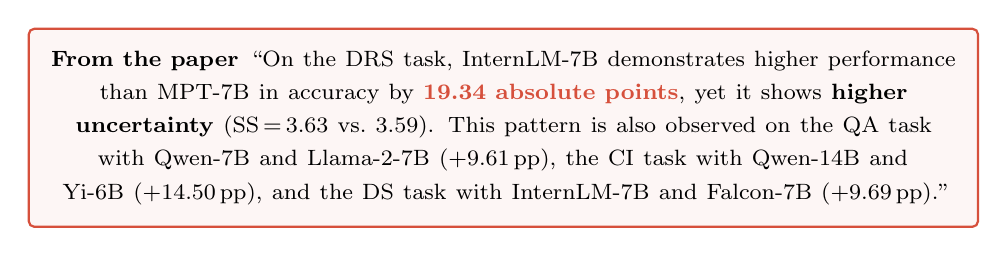
\begin{tikzpicture}
  \node[draw=Coral,line width=0.8pt,fill=Coral!5,
        inner sep=8pt,rounded corners=2pt,
        text width=\linewidth-18pt,align=center]{%
    \footnotesize
    \textbf{From the paper}\enspace
    ``On the DRS task, InternLM-7B demonstrates higher performance than MPT-7B in accuracy by
    \textcolor{Coral}{\bfseries 19.34 absolute points}, yet it shows \textbf{higher uncertainty} (SS\,=\,3.63 vs.\ 3.59).
    This pattern is also observed on the QA task with Qwen-7B and Llama-2-7B (+9.61\,pp),
    the CI task with Qwen-14B and Yi-6B (+14.50\,pp), and the DS task with InternLM-7B and Falcon-7B (+9.69\,pp).''
  };
\end{tikzpicture}

\vspace{0.45em}
\begin{columns}[T]
  \begin{column}{0.46\textwidth}
    {\small\bfseries\color{darkred}What SS actually measures}
    \hruleslide
    \begin{itemize}\setlength\itemsep{5pt}\footnotesize
      \item SS measures the \textbf{spread of the probability distribution}, not whether the predicted answer is correct.
      \item A model that often picks the correct answer but with a \emph{diffuse} distribution (e.g.\ $[0.25,0.23,0.20,\ldots]$) forces CP to include many options to guarantee coverage $\Rightarrow$ high SS.
      \item A model that is frequently wrong but \emph{very confident} (e.g.\ $[0.90,0.05,\ldots]$) produces small prediction sets $\Rightarrow$ low SS — even though it is less accurate.
    \end{itemize}
  \end{column}

  \begin{column}{0.02\textwidth}\color{Rule}\vrule\end{column}

  \begin{column}{0.46\textwidth}
    {\small\bfseries\color{darkred}Why it matters}
    \hruleslide
    \begin{itemize}\setlength\itemsep{5pt}\footnotesize
      \item ``The ranking of LLMs based on accuracy differs from that based on uncertainty, suggesting that some LLMs possessing higher accuracy actually display higher uncertainty.)
      \item ``Relying solely on accuracy for benchmarking LLMs is insufficient. It is imperative to take uncertainty into account.)
      \item \textbf{Accuracy} $\equiv$ average correctness.
        \textbf{SS} $\equiv$ trustworthiness of individual predictions.
    \end{itemize}
  \end{column}
\end{columns}
\end{frame}

% ===============================================================

\end{document} 